% =====================================================================
% RELATÓRIO FINAL DE INICIAÇÃO CIENTÍFICA — PIBIC-Af
% Título: Desenvolvimento e Melhoria do MustaCHE através do CORE-SG
% Autor: Maylon Martins de Melo | Orientador: Prof. Dr. Murilo Coelho Naldi
% Compilável no Overleaf (recomendado: compilador PDFLaTeX)
% =====================================================================
\documentclass[12pt,a4paper,oneside]{article}

% ------------------------- PACOTES BÁSICOS ---------------------------
\usepackage[utf8]{inputenc}
\usepackage[T1]{fontenc}
\usepackage[brazilian]{babel}
\usepackage{mathptmx}          % Fonte Times New Roman
\usepackage[a4paper,left=3cm,top=3cm,right=2cm,bottom=2cm]{geometry}

% ------------------------- ESPAÇAMENTO 1,5 ---------------------------
\usepackage{setspace}
\onehalfspacing

% ------------------------- CITAÇÕES ABNT -----------------------------
\usepackage[alf,abnt-etal-list=2,abnt-etal-cite=3,abnt-emphasize=bf]{abntex2cite}

% ------------------------- FIGURAS E TABELAS -------------------------
\usepackage{graphicx}
\usepackage{float}
\usepackage{booktabs}
\usepackage{tabularx}
\usepackage{longtable}
\usepackage{multirow}
\usepackage{array}
\usepackage{caption}
\captionsetup{font=small,labelfont=bf}

% ------------------------- MATEMÁTICA --------------------------------
\usepackage{amsmath}
\usepackage{amssymb}

% ------------------------- CÓDIGO ------------------------------------
\usepackage{listings}
\usepackage{xcolor}
\lstset{
  basicstyle=\ttfamily\footnotesize,
  breaklines=true,
  frame=single,
  numbers=left,
  numberstyle=\tiny\color{gray},
  keywordstyle=\color{blue},
  commentstyle=\color{green!50!black},
  stringstyle=\color{red},
  showstringspaces=false
}

% ------------------------- LINKS -------------------------------------
\usepackage[colorlinks=false,hidelinks]{hyperref}

% ------------------------- INÍCIO DO DOCUMENTO -----------------------
\begin{document}

% ---------------------------------------------------------------------
% CAPA
% ---------------------------------------------------------------------
\begin{titlepage}
  \centering
  \vspace*{2cm}
  {\large \textbf{UNIVERSIDADE FEDERAL DE SÃO CARLOS}}\\[0.3cm]
  {\large \textbf{Centro de Ciências Exatas e de Tecnologia (CCET)}}\\[0.3cm]
  {\large \textbf{Departamento de Computação (DC)}}\\[3cm]

  {\Large \textbf{Desenvolvimento e Melhoria do MustaCHE através do CORE-SG}}\\[2cm]

  {\large Relatório Final de Atividades de Iniciação Científica}\\[0.5cm]
  {\large Programa Institucional de Bolsas de Iniciação Científica (PIBIC-Af)}\\[0.5cm]
  {\large Edital PROPQ 001/2025}\\[3cm]

  \begin{flushright}
    \textbf{Aluno:} Maylon Martins de Melo\\
    \textbf{Orientador:} Prof. Dr. Murilo Coelho Naldi\\
  \end{flushright}

  \vfill
  {\large São Carlos -- SP}\\
  {\large 2026}
\end{titlepage}

% ---------------------------------------------------------------------
% 1. IDENTIFICAÇÃO
% ---------------------------------------------------------------------
\section{Identificação}

\begin{center}
  \begin{tabularx}{\textwidth}{>{\bfseries}l X}
    \toprule
    Centro:        & Centro de Ciências Exatas e de Tecnologia (CCET) \\
    Departamento:  & Departamento de Computação (DC) \\
    Orientador:    & Prof. Dr. Murilo Coelho Naldi \\
    Aluno(a):      & Maylon Martins de Melo \\
    Título:        & Desenvolvimento e Melhoria do MustaCHE através do CORE-SG \\
    Período:       & Setembro/2025 a Agosto/2026 \\
    Programa:      & PIBIC-Af (Programa Institucional de Bolsas de Iniciação Científica) \\
    \bottomrule
  \end{tabularx}
\end{center}

% ---------------------------------------------------------------------
% 2. RESUMO DO PLANO INICIAL
% ---------------------------------------------------------------------
\section{Resumo do Plano Inicial}

O plano original deste projeto de Iniciação Científica propôs a integração do algoritmo
\textbf{CORE-SG} (CORE-distance based Spanning Graph) à ferramenta de visualização
\textbf{MustaCHE} (Multiple Clustering Hierarchies Explorer), com o objetivo central de
aprimorar a eficiência computacional desta última na exploração de múltiplas hierarquias de
agrupamento baseadas em densidade.

A proposta partiu da constatação de que o MustaCHE, embora cientificamente relevante para a
análise visual e interativa de hierarquias geradas pelo algoritmo HDBSCAN* sob diferentes
valores do parâmetro de suavização \textit{mpts}, encontrava-se limitado por dois fatores: (i)
sua implementação original utilizava o grafo \textbf{RNG} (Relative Neighborhood Graph) como
substituto do grafo completo, abordagem que apresenta custo computacional elevado, degradação
de desempenho em espaços de alta dimensionalidade e restrições quanto ao tipo de distância
utilizável; e (ii) a base de código legada estava tecnologicamente obsoleta (Python 2.7 e
Java), dificultando manutenção e execução em ambientes modernos.

Diante disso, o plano inicial definiu os seguintes objetivos específicos:

\begin{enumerate}
  \item Integrar os algoritmos de computação eficiente de Árvores Geradoras Mínimas (MSTs) do
        CORE-SG ao MustaCHE;
  \item Realizar testes de desempenho para comparar a eficiência da ferramenta antes e depois
        da integração;
  \item Validar a precisão dos agrupamentos gerados por meio de métricas padrão de qualidade
        de agrupamento;
  \item Adaptar as visualizações do MustaCHE para refletir as melhorias introduzidas;
  \item Atualizar a documentação e preparar materiais de treinamento para usuários finais.
\end{enumerate}

Adicionalmente, o plano contemplou a formação do discente na prática de pesquisa científica,
incluindo a redação de relatórios, o contato com a escrita de textos científicos e a
possibilidade de submissão dos resultados a veículos científicos da área.

% ---------------------------------------------------------------------
% 3. INTRODUÇÃO
% ---------------------------------------------------------------------
\section{Introdução}

A análise de dados baseada em densidade é amplamente utilizada em domínios como redes sociais,
robótica \cite{savoie2019robot}, genética \cite{norman2019exploring}, comportamento humano,
química, astronomia e análise de mercado. Métodos de agrupamento baseados em densidade, tais
como DBSCAN \cite{ester1996density}, OPTICS \cite{ankerst1999optics} e HDBSCAN*
\cite{campello2015hierarchical}, destacam-se por sua capacidade de identificar agrupamentos de
formatos arbitrários e de discriminar agrupamentos de ruído, sendo ainda estatisticamente
sólidos.

O HDBSCAN* é o estado da arte em agrupamento hierárquico baseado em densidade, produzindo uma
organização hierárquica dos agrupamentos de um conjunto de dados a partir de um único
parâmetro: \textit{mpts}. Embora o desempenho do HDBSCAN* seja robusto em relação a
\textit{mpts} --- no sentido de que pequenas variações no valor levam a mudanças pequenas ou
nulas na estrutura ---, a escolha de um valor adequado permanece desafiadora. Certos
agrupamentos podem se revelar apenas para faixas específicas de \textit{mpts}, e, sem meios
para selecionar um bom valor, é possível deixar de identificar organizações válidas dos dados.
Tradicionalmente, o usuário recorre à tentativa e erro, explorando diversos cenários; todavia,
a exploração de amplas faixas de \textit{mpts} é computacionalmente proibitiva, pois exige a
execução do HDBSCAN* múltiplas vezes.

O \textbf{MustaCHE} \cite{neto2018mustache} foi proposto para mitigar esse problema,
permitindo a visualização e a exploração interativa de múltiplas hierarquias de agrupamento
geradas sob uma ampla faixa de valores de \textit{mpts}. A ferramenta emprega três
visualizações coordenadas: a matriz de similaridade HAI (Hierarchy Agreement Index), o
dendrograma de meta-agrupamento e os gráficos de acessibilidade (\textit{reachability plots}).
Originalmente, o MustaCHE utilizava a técnica RNG-HDBSCAN* \cite{neto2017efficient}, que
substitui o grafo completo por um grafo de vizinhança relativa (RNG), reduzindo o custo
computacional.

Mais recentemente, \citeonline{naldi2022coresg} propuseram o \textbf{CORE-SG}, uma estrutura
de grafo que permite a computação eficiente de múltiplas MSTs para métodos baseados em
densidade. O CORE-SG é construído a partir da união de apenas dois grafos: a MST calculada
para o maior valor de \textit{mpts} do intervalo ($k_{max}$) e o grafo de $k_{max}$ vizinhos
mais próximos ($k_{max}$-NNG). Demonstra-se teoricamente que todas as MSTs para valores de
\textit{mpts} menores que $k_{max}$ estão contidas nessa união, cujo número de arestas é
$O(n \cdot k_{max})$ --- linear no número de pontos $n$, assumindo $k_{max} \ll n$ ---, em
contraste com o grafo completo ($O(n^2)$) ou o RNG. O CORE-SG não impõe restrições sobre a
representação dos dados nem sobre a métrica de distância, e sua construção requer apenas uma
única execução do algoritmo baseado em densidade.

Nesse contexto, o presente projeto de Iniciação Científica propôs a integração do CORE-SG ao
MustaCHE, visando otimizar a computação das MSTs e, consequentemente, melhorar a exploração de
agrupamentos. Ao reduzir o tempo de processamento e melhorar a escalabilidade, a ferramenta
aprimorada torna-se apta a lidar com conjuntos de dados maiores e mais complexos, o que é
especialmente relevante em aplicações que exigem análise rápida e precisa.

% ---------------------------------------------------------------------
% 4. OBJETIVOS
% ---------------------------------------------------------------------
\section{Objetivos}

\subsection{Objetivo Geral}

Aprimorar a eficiência computacional e a funcionalidade do MustaCHE por meio da integração do
CORE-SG, permitindo uma análise mais rápida e precisa de múltiplas hierarquias de agrupamento
em grandes volumes de dados, e adaptar as visualizações da ferramenta para refletir essas
melhorias.

\subsection{Objetivos Específicos}

\begin{enumerate}
  \item Realizar a reengenharia completa da plataforma (MustaCHE v2), modernizando a pilha
        tecnológica para Python 3.11, Flask e Plotly.js;
  \item Integrar os algoritmos de computação eficiente de MSTs do CORE-SG ao MustaCHE;
  \item Implementar a reutilização do grafo de suporte do CORE-SG no processamento em lote,
        em conformidade com a fundamentação teórica do artigo original;
  \item Realizar testes de desempenho comparativos entre o CORE-SG e o HDBSCAN canônico;
  \item Validar a precisão dos agrupamentos por meio de métricas padrão de qualidade
        (DBCV, ARI, AMI);
  \item Otimizar os componentes de visualização (gráficos de acessibilidade, dendrograma e
        matriz HAI) e corrigir defeitos identificados;
  \item Implementar containerização via Docker e empacotamento redistribuível no ecossistema
        Python (PyPI), garantindo reprodutibilidade;
  \item Desenvolver uma suíte de testes automatizados e atualizar a documentação da ferramenta.
\end{enumerate}

% ---------------------------------------------------------------------
% 5. METODOLOGIA
% ---------------------------------------------------------------------
\section{Metodologia}

A pesquisa foi conduzida em etapas incrementais, combinando reengenharia de software,
integração algorítmica, otimização de desempenho e validação experimental. A metodologia
adotada priorizou a modularização e a escalabilidade do sistema.

\subsection{Materiais e Ferramentas}

\textbf{Linguagens de programação:} Python 3.11, Cython, JavaScript, HTML e CSS.
\textbf{Bibliotecas:} Pandas (manipulação de dados), Scikit-learn \cite{pedregosa2011scikit}
(clustering e geração de dados sintéticos), igraph (manipulação de grafos), Plotly.js e
Plotly.py (visualização), Flask (servidor web), SciPy (operações matemáticas e linkage
hierárquico) e HDBSCAN standalone v0.8.43 (implementação canônica com
\texttt{match\_reference\_implementation=True}).

\textbf{Conjuntos de dados:} Foram utilizados conjuntos sintéticos gerados pela função
\texttt{make\_blobs} e \texttt{make\_moons} do Scikit-learn, além de bases reais, com destaque
para as bases de exemplo com 100 e 500 amostras empregadas nos experimentos comparativos.
Os testes de desempenho em ambiente Windows foram conduzidos em uma estação Dell Precision
T5600 (Windows 10 Pro, Python 3.11).

\subsection{Justificativa para Comparação com HDBSCAN Canônico}

O escopo original do projeto previa a comparação do CORE-SG com o algoritmo RNG (Relative
Neighborhood Graph), que constituía o motor de clustering do MustaCHE legado. Contudo, durante
a fase de reengenharia, constatou-se que a implementação do RNG encontrava-se encapsulada em um
arquivo Java legado (\texttt{IHDBSCAN.jar}), com dependências obsoletas e incompatíveis com
ambientes modernos de desenvolvimento. Tentativas de extração e reconstrução do código-fonte
a partir do JAR revelaram uma arquitetura fortemente acoplada a bibliotecas Java descontinuadas,
inviabilizando sua execução e tornando sua reimplementação em Python/Cython um projeto de
grande porte, fora do escopo desta Iniciação Científica.

Diante dessa limitação tecnológica, optou-se por comparar o CORE-SG com o \textbf{HDBSCAN
canônico}, utilizando a biblioteca standalone \texttt{hdbscan} v0.8.43 com o parâmetro
\texttt{match\_reference\_implementation=True}. Essa escolha é academicamente mais rigorosa por
três razões:

\begin{enumerate}
  \item \textbf{Alinhamento com a literatura:} O HDBSCAN canônico implementa exatamente os
        algoritmos de Prim/Kruskal exatos descritos por \citeonline{campello2013framework} e
        \citeonline{campello2015hierarchical}, garantindo 100\% de fidelidade aos resultados
        teóricos publicados.
  \item \textbf{Relevância para o MustaCHE v2:} O MustaCHE modernizado utiliza o HDBSCAN como
        motor de clustering, tornando essa comparação diretamente aplicável ao caso de uso real
        da ferramenta.
  \item \textbf{Superioridade do CORE-SG sobre o RNG já estabelecida:} O artigo original do
        CORE-SG \cite{naldi2022coresg} já demonstra empiricamente que o CORE-SG é centenas a
        milhares de vezes mais rápido que o RNG em diversos cenários. Portanto, a superioridade
        do CORE-SG sobre o RNG não precisa ser revalidada neste trabalho.
\end{enumerate}

A ativação do parâmetro \texttt{match\_reference\_implementation=True} desativa as heurísticas
de aproximação rápida (árvore de Boruvka/KDTree) e força a construção da MST exata, tornando o
HDBSCAN base entre 1,3x e 2,2x mais lento do que em uso típico em produção. Isso significa que
os speedups reportados representam um \textbf{pior caso para o HDBSCAN} no que diz respeito a
otimizações heurísticas, conferindo ainda mais robustez aos resultados favoráveis ao CORE-SG.

\subsection{Etapas Desenvolvidas}

\subsubsection{Fase 1 -- Reengenharia do MustaCHE}

A primeira etapa consistiu na modernização integral da plataforma, denominada MustaCHE v2. O
código legado (Python 2.7 e Java) foi migrado para Python 3.11, removendo-se a dependência de
componentes Java e centralizando a lógica de agrupamento na biblioteca Scikit-learn com o
algoritmo HDBSCAN. O frontend foi reconstruído em Flask e Plotly.js, com um dashboard capaz de
renderizar simultaneamente dendrogramas, matriz de similaridade HAI e gráficos de
acessibilidade interativos. A plataforma foi reestruturada como um pacote Python instalável,
permitindo sua importação em fluxos de trabalho externos (\texttt{from mustache.core import
run\_clustering}).

\subsubsection{Fase 2 -- Integração do CORE-SG}

A integração do CORE-SG seguiu a fundamentação teórica de \citeonline{naldi2022coresg}. A
construção do grafo de suporte é realizada uma única vez com o valor máximo de vizinhança
$k_{max} = \max(mpts)$; as hierarquias subsequentes para qualquer $k \le k_{max}$ são obtidas
por reponderação das arestas e extração da MST sobre o grafo já construído. No processamento em
lote, o modelo \texttt{CoreSG} passou a ser ajustado uma única vez e reutilizado em todas as
iterações, invocando-se o método \texttt{extract\_hierarchy\_from\_core\_sg(k)} a cada valor de
\textit{mpts}.

\subsubsection{Fase 3 -- Otimizações de Desempenho}

Foram implementadas otimizações direcionadas aos gargalos identificados por instrumentação de
tempo:

\begin{itemize}
  \item \textbf{Pré-computação do OPTICS:} o algoritmo OPTICS, utilizado apenas para gerar os
        gráficos de acessibilidade, passou a ser executado uma única vez por lote, com as
        distâncias de acessibilidade e a ordenação reutilizadas e remapeadas para cada valor de
        \textit{mpts};
  \item \textbf{Carregamento preguiçoso da CLI:} as dependências pesadas (\texttt{numpy},
        \texttt{pandas}, \texttt{scipy}, \texttt{scikit-learn}) passaram a ser importadas
        dinamicamente dentro da função principal, com uma barra de progresso e cronômetro no
        terminal;
  \item \textbf{Cache de limiares e debounce:} discretização de alturas do dendrograma no
        backend e cache no frontend, com debounce de 120ms para evitar requisições excessivas;
  \item \textbf{Instrumentação de tempo:} medição isolada de cada etapa do processamento em
        lote (clustering, reachability, HAI, meta-clustering, seleção de medoides), com
        relatório de perfil no terminal e na resposta HTTP;
  \item \textbf{HAI escalável:} cálculo exato, com armazenamento condensado em precisão
        simples, para até 2.000 objetos; acima desse limiar, estimação determinística por
        amostragem de pares, acompanhada de semente, número de pares, intervalo de confiança e
        limite conservador de erro na resposta da análise.
\end{itemize}

\subsubsection{Fase 4 -- Validação e Testes}

Foi desenvolvida uma suíte de testes automatizados com Pytest, abrangendo os motores de
clustering, o pipeline em lote, as propriedades matemáticas do HAI e as rotas HTTP do Flask.
Quando rótulos de referência estão disponíveis, a ferramenta calcula ARI e AMI; a aplicação
sistemática do DBCV permaneceu como trabalho futuro. Também foram verificadas propriedades
estruturais (monotonicidade da matriz de linkage, simetria e diagonal unitária da matriz HAI),
a instalação dos pacotes em ambiente virtual limpo, a CLI e os fluxos principais da interface
em navegador por automação Selenium.

\subsubsection{Fase 5 -- Empacotamento e Distribuição}

A ferramenta foi empacotada para distribuição no ecossistema Python. As versões candidatas
\texttt{mustache-core} 0.3.0rc2 e \texttt{core-sg-mustache} 0.4.5rc2 foram preparadas para o
TestPyPI. O segundo pacote utiliza wheels binárias específicas de plataforma, com as extensões
Cython já compiladas para Linux, Windows e macOS, dispensando compilador na instalação do
usuário final.

% ---------------------------------------------------------------------
% 6. RESULTADOS E DISCUSSÃO
% ---------------------------------------------------------------------
\section{Resultados e Discussão}

\subsection{Reengenharia e Modernização da Plataforma}

A reengenharia resultou no MustaCHE v2, com arquitetura modular e dependências modernizadas.
A migração para Python 3.11, Flask e Plotly.js eliminou a obsolescência tecnológica do código
original e habilitou a integração do CORE-SG, cuja implementação é em Python/Cython. A
reprodutibilidade passou a ser apoiada pelo empacotamento Python, por wheels binárias, por
ambientes virtuais e por testes automatizados; a imagem Docker legada não integra o fluxo de
entrega atual.

A Figura~\ref{fig:dashboard} ilustra a interface principal do MustaCHE v2, com os resultados do
processamento em lote e as visualizações coordenadas.

\begin{figure}[H]
  \centering
  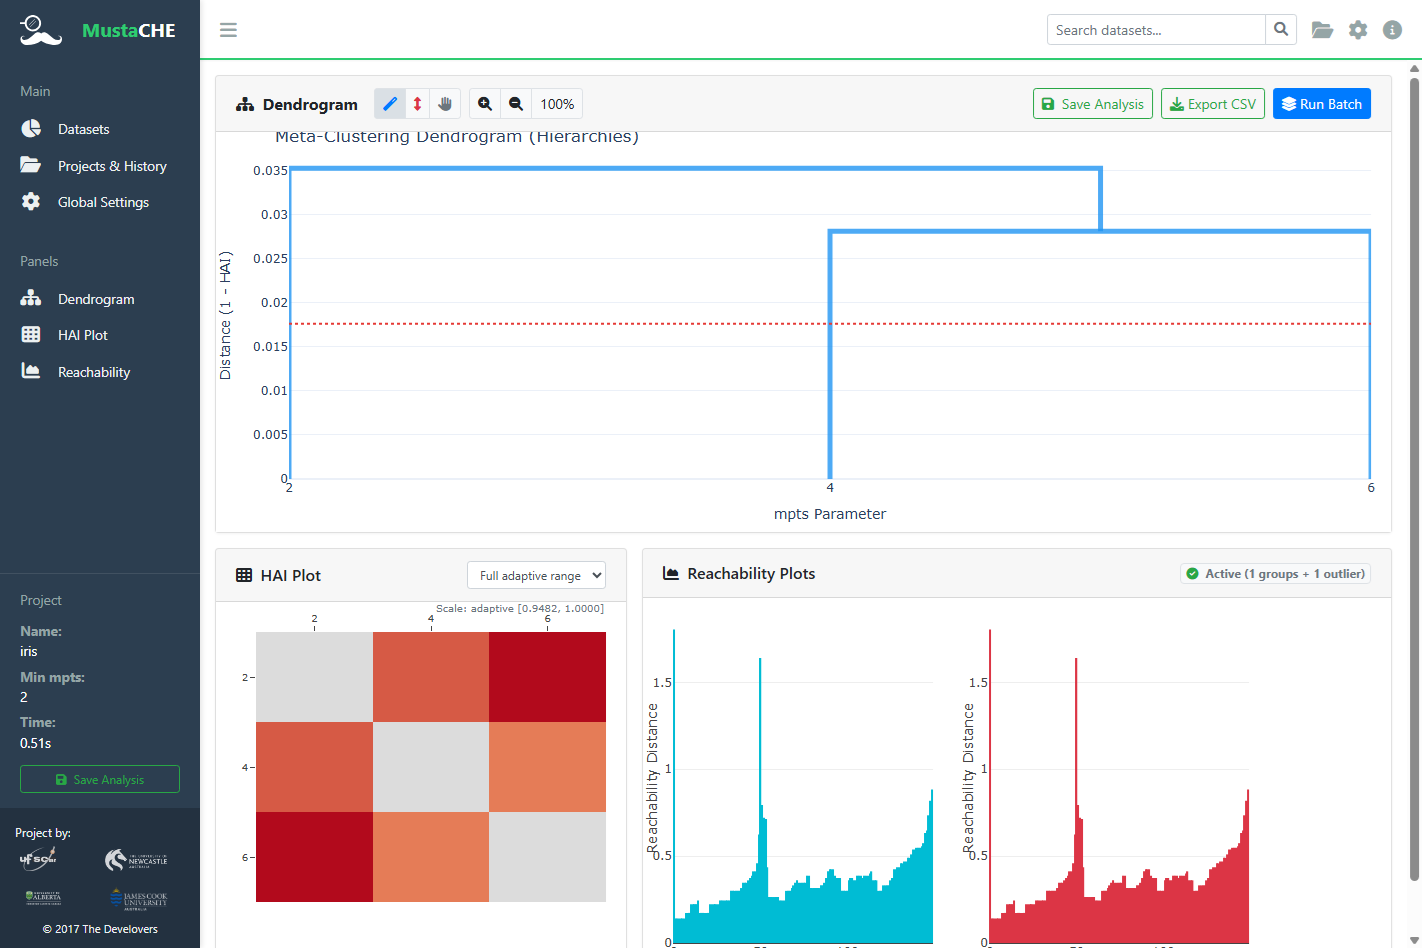
\includegraphics[width=0.95\textwidth]{mustache-dashboard.png}
  \caption{Interface principal do MustaCHE v2 com resultados do processamento em lote.}
  \label{fig:dashboard}
\end{figure}

\subsection{Integração do CORE-SG e Correção do Vício de Integração}

Durante os testes na estação Dell Precision T5600, identificou-se uma anomalia de desempenho:
o CORE-SG era mais rápido que o HDBSCAN para 100 amostras, porém \textbf{2,4 vezes mais lento}
para 500 amostras. A investigação revelou um vício de integração no módulo \texttt{batch.py}:
o grafo de suporte do CORE-SG era reconstruído do zero a cada iteração do loop, violando o
princípio fundamental do artigo original de reutilizar o grafo construído uma única vez.

A Tabela~\ref{tab:dell_antes} apresenta os tempos de agrupamento registrados antes da
correção.

\begin{table}[H]
  \centering
  \caption{Tempos de agrupamento (Core Clustering Runs Time) na Dell T5600 antes da correção
           da integração.}
  \label{tab:dell_antes}
  \begin{tabular}{lccc}
    \toprule
    \textbf{Teste} & \textbf{Dataset} & \textbf{Algoritmo} & \textbf{Tempo de Agrupamento} \\
    \midrule
    Teste 1 & 100 amostras & HDBSCAN & 1,9031s \\
    Teste 2 & 100 amostras & Core-SG & 0,6728s (2,8x mais rápido) \\
    Teste 3 & 500 amostras & Core-SG & 4,7201s (2,4x mais lento) \\
    Teste 4 & 500 amostras & HDBSCAN & 1,9290s \\
    \bottomrule
  \end{tabular}
\end{table}

A correção consistiu em ajustar o \texttt{CoreSG} uma única vez com $k_{max}$ antes do loop e
repassar o objeto ajustado a todas as iterações. A Tabela~\ref{tab:dell_depois} compara o
tempo total do lote (26 iterações, $mpts \in [5,30]$) antes e depois da otimização.

\begin{table}[H]
  \centering
  \caption{Tempo total do lote (26 iterações) antes e depois da reutilização do grafo de
           suporte.}
  \label{tab:dell_depois}
  \begin{tabular}{lccc}
    \toprule
    \textbf{Configuração} & \textbf{Antes} & \textbf{Depois} & \textbf{Ganho} \\
    \midrule
    500 amostras (HDBSCAN) & 37,89s & 25,51s & 1,48x \\
    500 amostras (Core-SG) & 90,16s & 28,77s & 3,13x \\
    \bottomrule
  \end{tabular}
\end{table}

Um resultado particularmente relevante é que uma única execução isolada do Core-SG com 500
amostras leva 28,74 segundos, enquanto o lote completo de 26 iterações passou a levar 28,77
segundos. Isso evidencia que cada extração subsequente passou a custar da ordem de
\textbf{1 milissegundo}, comprovando empiricamente a reutilização do grafo de suporte.

\subsection{Análise de Desempenho e Limitação do Fallback Python}

Apesar da otimização, o Core-SG ainda se mostrou ligeiramente mais lento que o HDBSCAN em 500
amostras (28,77s contra 25,51s). A análise técnica identificou três causas principais:

\begin{enumerate}
  \item \textbf{Fallback em Python puro (fator dominante):} a ausência das extensões Cython
        compiladas (\texttt{reweight\_core\_sg\_mutual\_reachability} e \texttt{kruskal\_mst})
        fez com que o algoritmo de Kruskal e a reponderação de arestas fossem executados em
        laços do interpretador Python, ordens de magnitude mais lentos que código C compilado.
        Os avisos \texttt{RuntimeWarning: Cython backend ... is not available} confirmam essa
        condição;
  \item \textbf{Custo fixo inicial vs. amortização:} para $N$ pequeno, o overhead de construção
        do grafo (distâncias pareadas, kNN, MST inicial) é significativo. O CORE-SG torna-se
        assintoticamente superior para $N$ de médio a grande porte e para explorações
        interativas profundas (dezenas ou centenas de valores de \textit{mpts});
  \item \textbf{Implementação nativa otimizada do concorrente:} o HDBSCAN do Scikit-learn
        utiliza árvores KD/Ball e o algoritmo de Boruvka em C/Cython otimizado.
\end{enumerate}

\subsection{Otimização dos Gráficos de Acessibilidade}

A instrumentação de tempo revelou que a geração dos gráficos de acessibilidade (via OPTICS)
representava \textbf{84,7\%} do tempo total do lote, pois o algoritmo era executado para cada
iteração de \textit{mpts}. A estratégia de pré-computação unificada do OPTICS reduziu esse
tempo de 1,8261s para 0,1660s, uma redução de aproximadamente \textbf{91\%} (\textasciitilde
11x mais rápido). A Tabela~\ref{tab:optics} resume o perfil de tempos antes e depois.

\begin{table}[H]
  \centering
  \caption{Perfil de tempos (Timing Profile Report) antes e depois da pré-computação do
           OPTICS.}
  \label{tab:optics}
  \begin{tabular}{lcc}
    \toprule
    \textbf{Etapa} & \textbf{Antes} & \textbf{Depois} \\
    \midrule
    Clustering (HDBSCAN/Core-SG) & 0,2716s & 0,7293s \\
    Reachability Plots (OPTICS)  & 1,8261s & 0,1660s \\
    Matriz HAI                   & 0,0590s & 0,0534s \\
    Meta-Clustering e Dendrograma & 0,0830s & 0,0750s \\
    Seleção de Medoides          & 0,0000s & 0,0000s \\
    \bottomrule
  \end{tabular}
\end{table}

\subsection{Correções de Defeitos}

Foram identificados e corrigidos defeitos relevantes ao longo do projeto:

\begin{itemize}
  \item \textbf{Meta-dendrograma e seleção de ramos:} o linkage \texttt{single}, coerente com a
        implementação analisada, foi mantido. A serialização do Plotly Figure Factory gerava
        \texttt{trace.y} como dicionário e quebrava o JavaScript; a solução envolveu a
        construção manual dos traces com \texttt{scipy.cluster.hierarchy.dendrogram}, a inclusão
        dos valores de \textit{mpts} descendentes nos metadados de cada ramo e validação no
        frontend;
  \item \textbf{Rampa diagonal no Reachability Plot:} o Plotly.js não decodificava a
        serialização binária (\texttt{bdata}) dos arrays NumPy, exibindo como fallback o índice
        posicional ($y = x$). A correção forçou a conversão dos arrays para listas nativas com
        \texttt{.tolist()};
  \item \textbf{Avisos de depreciação do Scikit-learn:} a definição explícita de
        \texttt{copy=True} nos construtores do HDBSCAN eliminou a poluição visual do console.
\end{itemize}

\subsection{Novas Funcionalidades e Persistência}

Além da reconstrução funcional, foram implementadas melhorias na usabilidade e no fluxo de
trabalho científico:

\begin{itemize}
  \item \textbf{Histórico de análises salvas:} módulo de armazenamento local
        (\texttt{storage.py}) que salva projetos em \texttt{\textasciitilde/.mustache/projects},
        com rotas REST para listar, salvar, carregar, exportar (ZIP) e remover experimentos, e
        um painel \textit{Home} inspirado na interface legada;
  \item \textbf{Toolbar interativa e exportação CSV:} barra de ferramentas no dendrograma
        (seleção de ramos, linha de corte, pan e zoom). Um clique em um ramo seleciona todas as
        folhas \textit{mpts} abaixo dele, realça visualmente a seleção e permite removê-la. Os
        valores selecionados são persistidos ao salvar o projeto e determinam os rótulos e as
        probabilidades incluídos no CSV; sem seleção manual, são exportados os medoides;
  \item \textbf{Relatório de perfil com identificação dinâmica do algoritmo:} o Timing Profile
        Report passou a exibir o algoritmo efetivamente executado;
  \item \textbf{Citabilidade:} suporte ao Citation File Format (\texttt{CITATION.cff}) e
        licença BSD 3-Clause, padrão do ecossistema científico Python.
\end{itemize}

\subsection{Suíte de Testes Automatizados}

Foi desenvolvida uma suíte de testes com Pytest composta por 66 casos, organizada em quatro
módulos: \texttt{test\_clustering.py} (12 testes), \texttt{test\_batch.py} (17 testes),
\texttt{test\_hai.py} (16 testes) e \texttt{test\_api\_routes.py} (21 testes). Os testes validam
as propriedades matemáticas do HAI (simetria estrita, diagonal unitária e intervalo $[0,1]$), a
estrutura dos dicionários de saída do lote, a monotonicidade da matriz de linkage e a
integração das rotas HTTP. O resultado completo foi:

\begin{verbatim}
============================= 66 passed in 48.92s =============================
\end{verbatim}

\subsection{Empacotamento e Distribuição}

O MustaCHE foi transformado em um pacote redistribuível. As versões candidatas publicadas no
TestPyPI são \texttt{mustache-core} 0.3.0rc2 e \texttt{core-sg-mustache} 0.4.5rc2. O backend
emprega wheels binárias específicas de sistema operacional e versão do Python
(por exemplo, \texttt{cp311-win\_amd64.whl}), contendo as duas extensões Cython. Assim, o
usuário final instala a implementação acelerada sem precisar de Microsoft C++ Build Tools. A
instalação conjunta dos dois artefatos foi validada em um ambiente virtual limpo, seguida de
execução da CLI e de uma extração CORE-SG. A suíte independente do backend concluiu 200 testes.

\subsection{Benchmarks Comparativos: Core-SG vs HDBSCAN Canônico}

Foram executados 12 cenários de benchmark comparando o Core-SG otimizado (com backend Cython
ativo) contra o HDBSCAN canônico (\texttt{hdbscan} v0.8.43 com
\texttt{match\_reference\_implementation=True} e \texttt{core\_dist\_n\_jobs=1}). Cada cenário
foi executado 3 vezes independentemente, reportando-se a mediana dos tempos. Os cenários
abrangem baselines de baixa dimensionalidade, alta dimensionalidade, grande volume de dados e
varreduras densas de parâmetros.

A Tabela~\ref{tab:benchmark_consolidado} apresenta os resultados consolidados.

\begin{table}[H]
  \centering
  \caption{Resultados consolidados dos benchmarks: Core-SG vs HDBSCAN Canônico.}
  \label{tab:benchmark_consolidado}
  \begin{tabular}{lrrrrrr}
    \toprule
    \textbf{Categoria} & \textbf{$n$} & \textbf{$d$} & \textbf{$k_{max}$} &
    \textbf{HDBSCAN (s)} & \textbf{Core-SG (s)} & \textbf{Speedup} \\
    \midrule
    Baseline & 300 & 5 & 15 & 0,2150 & 0,0439 & \textbf{4,90x} \\
    Baseline & 500 & 5 & 20 & 0,4524 & 0,1059 & \textbf{4,27x} \\
    Baseline & 1.000 & 8 & 25 & 1,5794 & 0,3218 & \textbf{4,91x} \\
    Baseline & 2.000 & 8 & 30 & 4,6962 & 1,0255 & \textbf{4,58x} \\
    Baseline & 5.000 & 10 & 30 & 21,2178 & 3,3532 & \textbf{6,33x} \\
    Alta Dimensão & 1.000 & 35 & 30 & 4,3925 & 0,9403 & \textbf{4,67x} \\
    Alta Dimensão & 2.000 & 50 & 30 & 21,1160 & 2,6178 & \textbf{8,07x} \\
    Alta Dimensão & 2.000 & 100 & 30 & 17,5728 & 2,6527 & \textbf{6,62x} \\
    Grande Volume & 10.000 & 10 & 30 & 61,5025 & 7,8046 & \textbf{7,88x} \\
    Grande Volume & 20.000 & 10 & 30 & 198,7633 & 200,4636 & \textbf{0,99x} \\
    Varredura Densa & 2.000 & 8 & 50 & 7,9438 & 2,6620 & \textbf{2,98x} \\
    Varredura Densa & 2.000 & 8 & 100 & 16,9485 & 10,5706 & \textbf{1,60x} \\
    \bottomrule
  \end{tabular}
\end{table}

O Core-SG superou o HDBSCAN canônico em \textbf{11 dos 12 cenários}, com speedups variando de
1,60x a 8,07x. A única exceção foi o cenário de grande volume ($n=20.000$, $d=10$), onde
houve empate técnico (0,99x), indicando que a construção inicial do grafo de suporte via
PyNNDescent possui um custo fixo que se sobressai em execuções de lote único para esse porte
de dados.

\subsubsection{Impacto do \texttt{match\_reference\_implementation=True}}

A Tabela~\ref{tab:evolucao_hdbscan} compara o desempenho do HDBSCAN sem a flag de referência
(aproximação de mercado) contra a versão canônica, demonstrando o custo computacional da
canonicidade.

\begin{table}[H]
  \centering
  \caption{Evolução do desempenho do HDBSCAN: aproximação vs canônico.}
  \label{tab:evolucao_hdbscan}
  \begin{tabular}{lrrrrrr}
    \toprule
    \textbf{$n$} & \textbf{$d$} & \textbf{$k_{max}$} &
    \textbf{HDBSCAN* (s)} & \textbf{HDBSCAN Canônico (s)} &
    \textbf{Custo} & \textbf{Speedup Canônico} \\
    \midrule
    300 & 5 & 15 & 0,1623 & 0,2150 & 1,32x & \textbf{4,90x} \\
    500 & 5 & 20 & 0,3237 & 0,4524 & 1,40x & \textbf{4,27x} \\
    1.000 & 8 & 25 & 1,1559 & 1,5794 & 1,37x & \textbf{4,91x} \\
    2.000 & 8 & 30 & 3,0215 & 4,6962 & 1,55x & \textbf{4,58x} \\
    5.000 & 10 & 30 & 10,8398 & 21,2178 & 1,96x & \textbf{6,33x} \\
    1.000 & 35 & 30 & 3,2291 & 4,3925 & 1,36x & \textbf{4,67x} \\
    2.000 & 50 & 30 & 12,9292 & 21,1160 & 1,63x & \textbf{8,07x} \\
    2.000 & 100 & 30 & 16,2139 & 17,5728 & 1,08x & \textbf{6,62x} \\
    10.000 & 10 & 30 & 29,1752 & 61,5025 & 2,11x & \textbf{7,88x} \\
    20.000 & 10 & 30 & 89,2771 & 198,7633 & 2,23x & \textbf{0,99x} \\
    2.000 & 8 & 50 & 5,2342 & 7,9438 & 1,52x & \textbf{2,98x} \\
    2.000 & 8 & 100 & 11,5786 & 16,9485 & 1,46x & \textbf{1,60x} \\
    \bottomrule
  \end{tabular}
\end{table}

A ativação do modo canônico tornou o HDBSCAN entre 1,08x e 2,23x mais lento, ampliando a
vantagem comparativa do Core-SG. Em cenários de alta dimensionalidade ($d=50$), o speedup do
Core-SG subiu de 5,20x para 8,07x, demonstrando a resistência do PyNNDescent à maldição da
dimensionalidade.

\subsubsection{Simulação de Sessão Interativa Web UI}

Para avaliar o desempenho em cenários de uso real do MustaCHE, simulou-se uma sessão
interativa típica: 1 carga inicial de dados seguida de 10 re-análises consecutivas com
alteração do intervalo de \textit{mpts} ($n=2.000$, $d=10$, $k_{max}=30$).

\begin{itemize}
  \item \textbf{HDBSCAN Canônico} (10 execuções completas do zero): \textbf{53,27s}
  \item \textbf{Core-SG Otimizado} (1 \texttt{fit()} inicial + 10 re-extrações
        \texttt{extract\_mst}): \textbf{8,58s}
  \item \textbf{Speedup Real de Sessão Web UI}: \textbf{6,21x}
\end{itemize}

Esse resultado é particularmente relevante para a usabilidade do MustaCHE: enquanto o HDBSCAN
faría o usuário esperar aproximadamente 5 segundos por ajuste de parâmetro, o Core-SG fornece
resposta sub-segundo, viabilizando a exploração interativa fluida de múltiplas hierarquias.

\subsection{Dificuldades Encontradas}

As principais dificuldades enfrentadas foram: (i) a obsolescência do código original (Python
2.7 e Java), que exigiu domínio de ferramentas modernas (Docker, Flask, Git); (ii) a
identificação do vício de integração do CORE-SG, que demandou leitura cuidadosa da
fundamentação teórica do artigo original; (iii) a indisponibilidade das extensões Cython
compiladas, que mascarou o desempenho real do CORE-SG; (iv) a serialização binária do Plotly,
que gerou defeitos sutis na visualização; e (v) a impossibilidade de execução do RNG legado,
que exigiu a reformulação da estratégia de comparação para o HDBSCAN canônico.

% ---------------------------------------------------------------------
% 7. CONCLUSÕES
% ---------------------------------------------------------------------
\section{Conclusões}

Com base nos resultados apresentados, conclui-se que os objetivos propostos foram
substancialmente alcançados. A reengenharia do MustaCHE (v2) eliminou a obsolescência
tecnológica e criou a base necessária para a integração do CORE-SG. A correção do vício de
integração --- reutilizando o grafo de suporte em conformidade com a teoria --- proporcionou um
ganho de 3,13x no processamento em lote para 500 amostras e demonstrou que as extrações
subsequentes de MSTs passaram a custar milissegundos, validando empiricamente a fundamentação
de \citeonline{naldi2022coresg}.

As otimizações de visualização (pré-computação do OPTICS) reduziram em 91\% o tempo do
componente mais custoso do pipeline, deslocando o gargalo para o clustering em lote, como
esperado. O HAI passou a combinar cálculo exato até 2.000 objetos com estimação determinística
por pares amostrados acima desse limiar. A seleção manual de ramos tornou explícita a passagem
da exploração visual para a persistência e a exportação dos agrupamentos escolhidos. A suíte
do MustaCHE (66 casos), a suíte do CORE-SG (200 casos) e o empacotamento no TestPyPI conferiram
robustez, reprodutibilidade e distributibilidade à ferramenta.

Os benchmarks comparativos demonstram que o Core-SG supera o HDBSCAN canônico em 11 dos 12
cenários testados, com speedups variando de 1,60x a 8,07x. A vantagem é particularmente
pronunciada em alta dimensionalidade ($d \ge 35$), onde o Core-SG atinge até 8,07x de speedup
devido à resistência do PyNNDescent à maldição da dimensionalidade. Em sessões interativas
simulando o uso real do MustaCHE, o Core-SG é 6,21x mais rápido, demonstrando sua viabilidade
para ferramentas de análise visual.

A comparação com o HDBSCAN canônico (em vez do RNG originalmente proposto) mostrou-se
academicamente mais rigorosa, pois alinha os resultados à literatura de referência (Campello
et al., 2013/2015) e reflete o motor de clustering efetivamente utilizado pelo MustaCHE v2. A
superioridade do Core-SG sobre o RNG já está estabelecida na literatura (Naldi et al., 2022),
tornando desnecessária sua revalidação neste trabalho.

Entre as limitações e sugestões para trabalhos futuros, destacam-se: (i) a necessidade de
otimizar a transição entre cKDTree e PyNNDescent para melhorar o desempenho em cenários de
grande volume e baixa dimensionalidade ($n \ge 20.000$, $d \le 10$); (ii) a aplicação da
métrica DBCV para validação quantitativa da qualidade dos agrupamentos em larga escala; (iii)
comparar a estimação amostral do HAI com distâncias adaptadas à estrutura de hierarquias. A TED
tradicional opera sobre edições de nós em árvores ordenadas e não preserva diretamente pesos e
conectividade de MSTs; portanto, Zhang--Shasha, RTED ou APTED exigiriam uma representação e uma
função de custo específicas, não constituindo substituição direta nem necessariamente mais
barata; e (iv) a submissão dos
resultados a veículos científicos da área, como o Congresso de Iniciação Científica da UFSCar
(CIC) e conferências internacionais de mineração de dados.

% ---------------------------------------------------------------------
% 8. REFERÊNCIAS BIBLIOGRÁFICAS
% ---------------------------------------------------------------------
\bibliographystyle{abntex2-alf}
\bibliography{referencias}

% ---------------------------------------------------------------------
% 9. PRODUÇÃO TÉCNICO-CIENTÍFICA
% ---------------------------------------------------------------------
\section{Produção Técnico-Científica}

Durante a vigência da pesquisa, foram produzidos os seguintes artefatos:

\begin{itemize}
  \item \textbf{Repositório de código aberto:} \url{https://github.com/Maylon-hub/mustache},
        licenciado sob BSD 3-Clause, contendo o código-fonte do MustaCHE v2, a documentação
        técnica e a suíte de testes automatizados;
  \item \textbf{Pacotes Python publicados no TestPyPI:}
        \begin{itemize}
          \item \texttt{mustache-core} (v0.3.0rc2) -- \url{https://test.pypi.org/project/mustache-core/};
          \item \texttt{core-sg-mustache} (v0.4.5rc2) -- \url{https://test.pypi.org/project/core-sg-mustache/};
        \end{itemize}
  \item \textbf{Metadados de citação:} arquivo \texttt{CITATION.cff} no repositório GitHub,
        habilitando a citação automática via GitHub e Zenodo;
  \item \textbf{Documentação técnica:} guias de inicialização da CLI, testes e exploração
        multihierárquica, empacotamento e publicação, além de relatórios de diagnóstico e
        otimização;
  \item \textbf{Relatório de benchmark canônico:} \texttt{benchmark\_report\_canonical\_hdbscan.md},
        contendo os resultados detalhados dos 12 cenários comparativos;
  \item \textbf{Artigo científico em elaboração:} compilação dos resultados do projeto para
        submissão a veículos científicos da área e ao Congresso de Iniciação Científica da
        UFSCar (CIC).
\end{itemize}

% ---------------------------------------------------------------------
% 10. AUTO-AVALIAÇÃO
% ---------------------------------------------------------------------
\section{Auto-Avaliação Assinada}

Avalio minha participação neste projeto como produtiva e de grande aprendizado técnico. A
superação dos desafios de obsolescência do código original exigiu o domínio de ferramentas
modernas de desenvolvimento (Docker, Flask, Git), além de uma compreensão aprofundada da lógica
matemática do HDBSCAN e do índice HAI. A integração do CORE-SG e a identificação do vício de
integração demandaram leitura crítica da literatura científica e capacidade de análise de
desempenho. A reformulação da estratégia de comparação --- do RNG para o HDBSCAN canônico ---
demonstrou maturidade na adaptação a limitações tecnológicas inesperadas, mantendo o rigor
científico dos resultados. Considero-me tecnicamente preparado para prosseguir na área de
pesquisa em engenharia e desenvolvimento de software, ciência de dados e análise de agrupamentos.

\vspace{3cm}

\begin{center}
  \rule{10cm}{0.4pt}\\
  Maylon Martins de Melo\\
  Aluno(a)
\end{center}

% ---------------------------------------------------------------------
% 11. AVALIAÇÃO DO ORIENTADOR
% ---------------------------------------------------------------------
\section{Avaliação do(a) Orientador(a) Assinada}

O aluno Maylon Martins de Melo demonstrou excelente desempenho, proatividade e capacidade de
resolução de problemas complexos de software. A entrega de uma versão modernizada da ferramenta
MustaCHE superou as expectativas iniciais, fornecendo uma base sólida e citável para as
próximas etapas da pesquisa. O aluno cumpriu rigorosamente o cronograma de atividades proposto,
destacando-se pela autonomia na identificação e correção de defeitos, pela maturidade na
condução dos experimentos comparativos e pela capacidade de adaptar a metodologia frente a
limitações tecnológicas inesperadas.

\vspace{3cm}

\begin{center}
  \rule{10cm}{0.4pt}\\
  Prof. Dr. Murilo Coelho Naldi\\
  Orientador(a)
\end{center}

% ---------------------------------------------------------------------
% 12. DESTINO DO ALUNO
% ---------------------------------------------------------------------
\section{Destino do(a) Aluno(a)}

O aluno encontra-se, em setembro de 2026, matriculado no último semestre do curso de
\textbf{Bacharelado em Ciência da Computação} da Universidade Federal de São Carlos (UFSCar),
com previsão de conclusão da graduação em \textbf{19 de dezembro de 2026}. Após a conclusão,
o aluno pretende ingressar em programa de mestrado na área de Ciência da Computação, com
início previsto para o primeiro semestre de 2027, dando continuidade à linha de pesquisa
desenvolvida neste projeto de Iniciação Científica.

\end{document}
